% vim: set tw=78 sts=2 sw=2 ts=8 aw et ai:
\documentclass{workshop}

% Comentează liniile de mai jos în cazul în care nu există cod de inclus.
\usepackage{code/highlight}
\usepackage{color}        % dacă e folosit highlight
\usepackage{alltt}        % dacă e folosit highlight

\title[Sesssion 1]{Session 1}
\subtitle{Getting started with the Linux Kernel}
\author{Daniel Băluță, Irina Preșa}
\date{02 July 2012}

\begin{document}

% Arătăm numărul frame-ului
\setbeamertemplate{footline}[frame number]

\frame{\titlepage}

% NB: Secțiunile nu sunt marcate vizual, ci doar apar în cuprins
\section{Introduction}

\begin{frame}{Motivation}
	\begin{itemize}
	\item Linux is everywhere
	\begin{itemize}
		\item 800k phones, 700k TVs activated daily
		\item Google, Twitter, Facebook, Amazon
		\item 9 out of 10 of the world's super computers
	\end{itemize}
	\item open source
	\item top-notch programmers
	\item personal recognition
	\item fun, a lot of fun
	\end{itemize}
\end{frame}
\begin{frame}{What is a kernel?}
	\begin{itemize}
	\item central piece of an operating system
	\item hardware control
	\item resource management
	\item application support
	\end{itemize}
\end{frame}

\begin{frame}{History}
	\begin{itemize}
	\item 1964 - Multics, MIT
	\item 1969 - Unics, Bell Labs
	\item 1983 - GNU Project
	\item 1991 - Linux
	\end{itemize}
\end{frame}


\section{Source Code Browsing}

\begin{frame}{Source Code Browsing}
\begin{figure}
  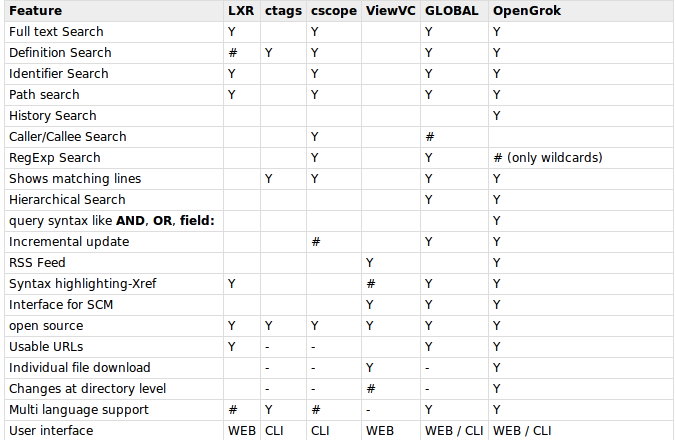
\includegraphics[scale=0.35]{img/source.png}
\end{figure}
\end{frame}

\section{Booting and Initialization}
\subsection{Intro: Controllers and Hardware}
\begin{frame}{Intro: Controllers and Hardware}
     \begin{figure}
         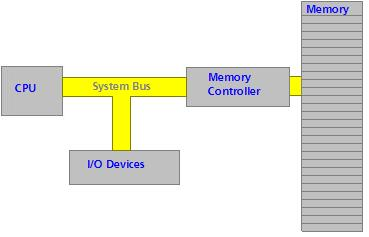
\includegraphics[scale=0.9]{img/bus.jpg}
      \end{figure}
\end{frame}

\begin{frame}{Intro: Controllers and Hardware}
\textbf{Real Mode}\\
\begin{itemize}
  \item CPU puts \textbf{physical} address on the bus.
  \item the memory controller recognizes it.
\end{itemize}

\textbf{Protected Mode}\\
\begin{itemize}
  \item CPU puts \textbf{virtual} address on the bus.
  \item MMU translates it into a physical address.
  \item memory protection.
  \begin{itemize}
    \item 4 Operating Modes: Ring 0, Ring 1, Ring 2, Ring 3.
  \end{itemize}
  \item hardware support for virtual memory.
  \item can address more memory.
\end{itemize}
\end{frame}

\begin{frame}{Intro: Controllers and Hardware}
\textbf{I/O Ports}\\
\begin{itemize}
  \item device controller listens on its ports.
  \item CPU puts port on the bus and sets the I/O access line.
  \item the controller of the associated device recognizes it.
  \item the memory controller will ignore the address.
  \item CPU offers IN/OUT instructions.
  \item ex: Intel interrupt controller.
\end{itemize}

\textbf{Memory Mapped I/O}\\
\begin{itemize}
  \item device controller mapped into memory.
  \item CPU puts address on the bus.
  \item the memory controller recognizes it.
  \item ex: ARM interrupt controller.
\end{itemize}
\end{frame}

\subsection{Before Kernel}
\begin{frame}{Before Kernel}
      \begin{figure}
         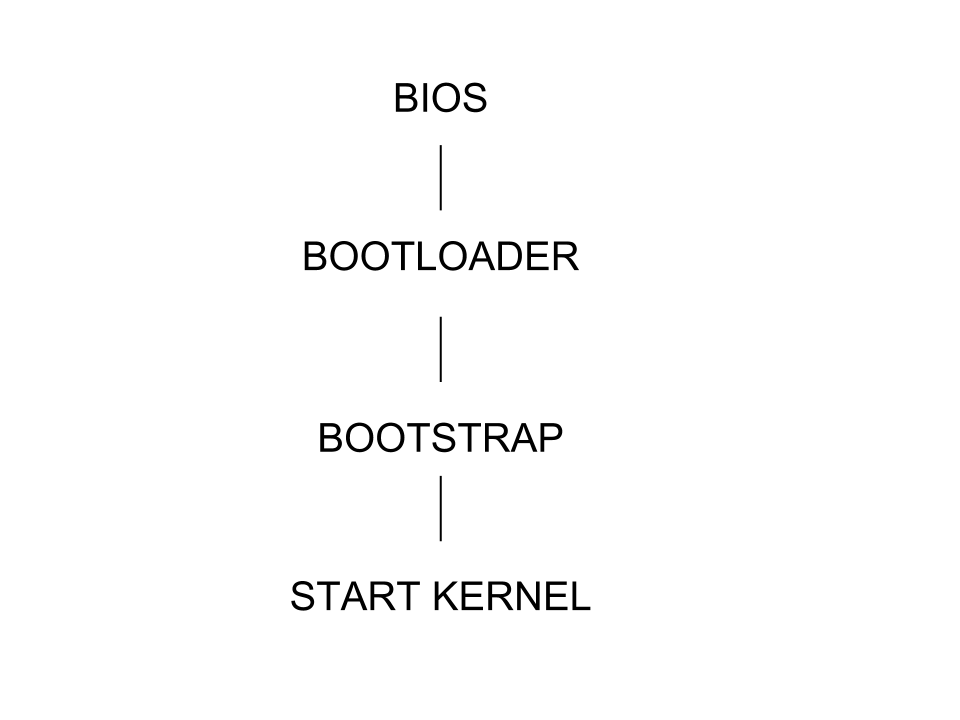
\includegraphics[scale=0.3]{img/boot.png}
      \end{figure}
\end{frame}

\begin{frame}{BIOS}
\begin{itemize}
\item POST : Performs the Power On Self Tests.
\item basic devices initialization (needed for the boot process).
\item creates Real Mode memory map.
\item finds the boot device and jumps to its sector '0' (load MBR).
\end{itemize}
\end{frame}

%TODO: de ce mai fol bootloader?
\begin{frame}{Bootloader}
\begin{itemize}
\item loads the operating system (can boot more than one OS).
\item it looks in the /boot directory and loads the kernel image.
\end{itemize}
\end{frame}

\begin{frame}{Bootstrap}
\begin{itemize}
\item assembly code added to the kernel image (bzImage).
\item uncompress the image ("Decrompressing Linux...").
\item call start\_kernel function.
\end{itemize}
\end{frame}

\begin{frame}{Extra: U-Boot}
      \begin{figure}
         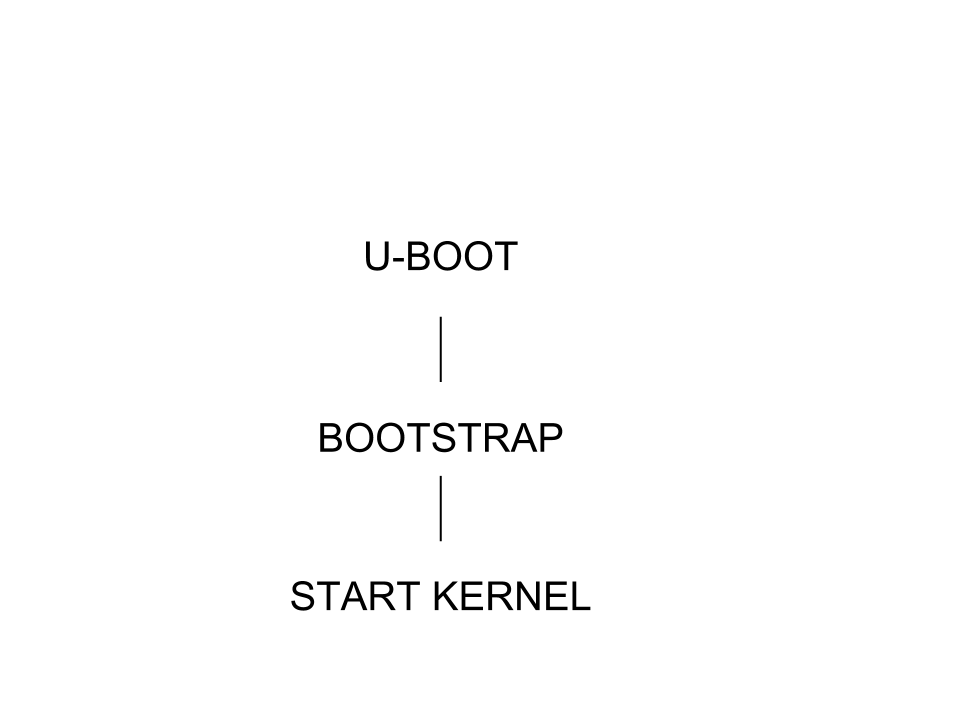
\includegraphics[scale=0.3]{img/u-boot.png}
      \end{figure}
\end{frame}

\begin{frame}{Extra: U-Boot}
\begin{itemize}
\item universal bootloader.
\item network and serial line configurations.
\item can load kernel image into memory (RAM).
  \begin{itemize}
  \item from the network (tftp), sdcard or flash memory.
  \end{itemize}
\end{itemize}
\end{frame}

\begin{frame}{Extra: Boot Embedded Device}
  \begin{columns}
    \begin{column}[l]{0.45\textwidth}
      \begin{figure}
         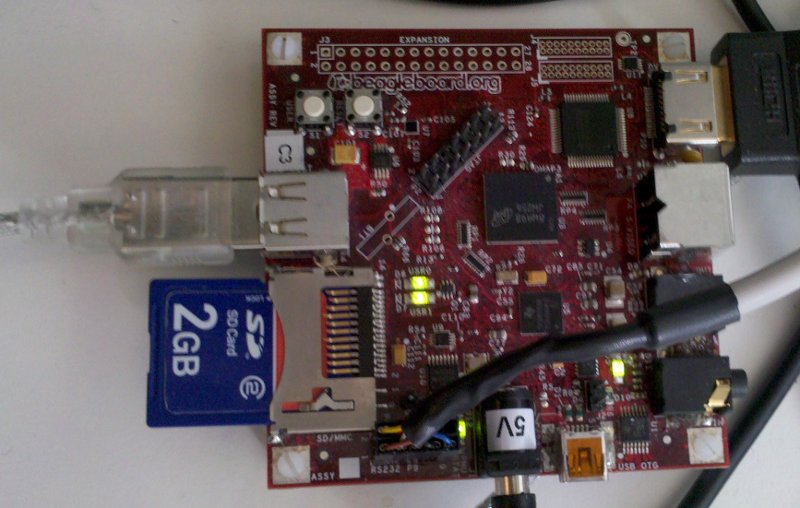
\includegraphics[scale=0.17]{img/beagle.jpg}
      \end{figure}
    \end{column}
    \begin{column}[l]{0.45\textwidth}
      \begin{figure}
         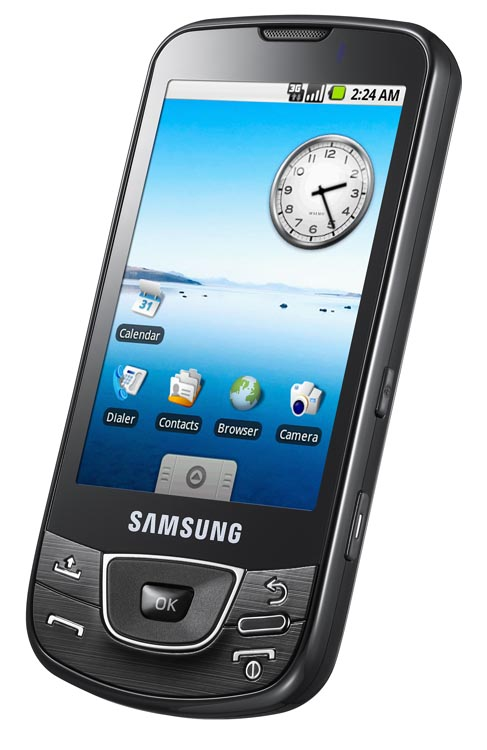
\includegraphics[scale=0.65]{img/phone.jpg}
      \end{figure}
    \end{column}
  \end{columns}
\end{frame}

\begin{frame}{Extra: Case Study - Boot Embedded Device}
  \begin{columns}
    \begin{column}[l]{0.45\textwidth}
      \begin{figure}
         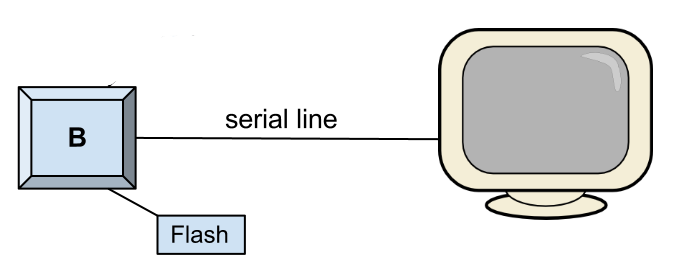
\includegraphics[scale=0.17]{img/flash.png}
      \end{figure}
      \begin{center}
        \tiny{- burn u-boot and kernel images on the flash.}
      \end{center}
    \end{column}
    \pause
    \begin{column}[l]{0.45\textwidth}
      \begin{figure}
         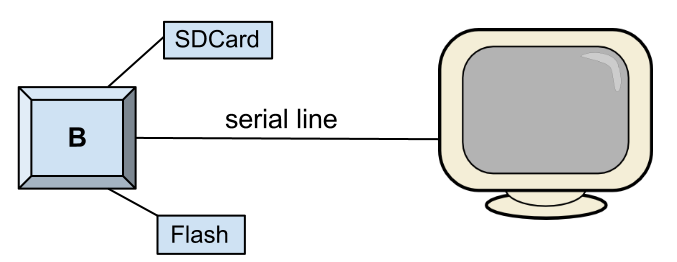
\includegraphics[scale=0.17]{img/sdcard.png}
      \end{figure}
      \begin{center}
        \tiny{- fatload mmc 0 8000 image.bin}
      \end{center}
    \end{column}
  \end{columns}
     \pause
     \begin{figure}
         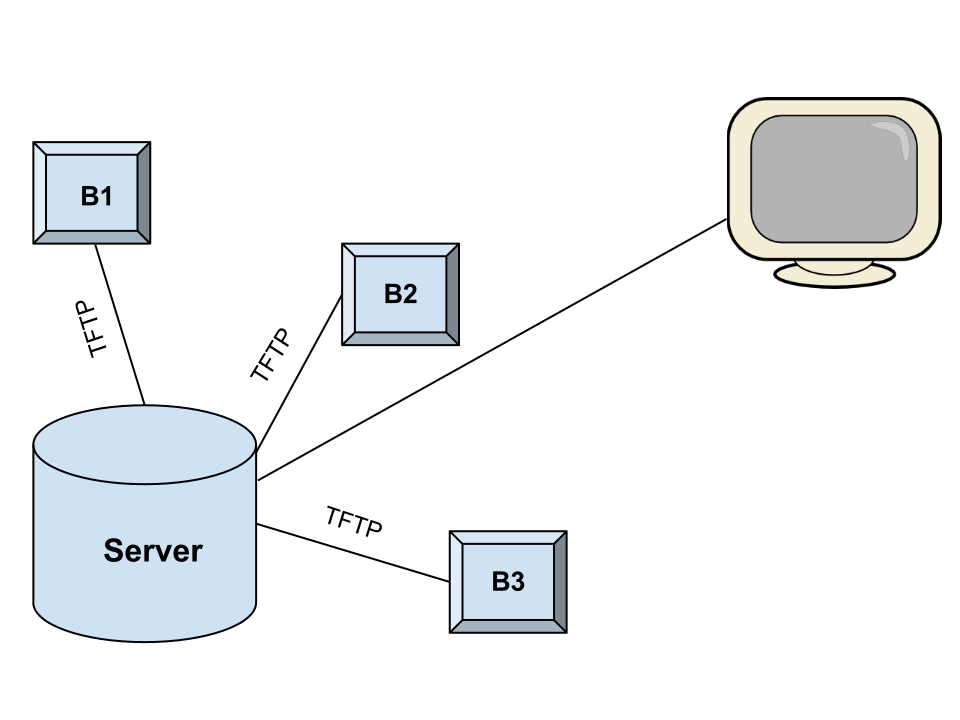
\includegraphics[scale=0.17]{img/complex.png}
      \end{figure}
      \begin{center}
      \tiny{- tftp 8000 image.bin}
      \end{center}
\end{frame}


\subsection{Startup Kernel}

\begin{frame}{Startup Kernel}

\textbf{Entry point...}\\
\begin{itemize}
\item startup\_32
\begin{itemize}
\item page tables
\item enable mmu
\end{itemize}
\end{itemize}

\textbf{Initialize...}\\
\begin{itemize}
\item start\_kernel
\begin{itemize}
\item trap\_init
\item mm\_init
\item init\_IRQ
\item sched\_init
\item time\_init
\item console\_init
\item smp\_init
\end{itemize}
\end{itemize}

\textbf{And.. UP!}\\
\begin{itemize}
\item rest\_init
\begin{itemize}
\item kernel\_thread
\item cpu\_idle
\end{itemize}
\end{itemize}
\end{frame}

%//TODO: kernel thread si cpu idle code??
\begin{frame}[fragile]{Enable Paging}
\input{code/paging}
\end{frame}

\begin{frame}[fragile]{Init Traps}
\input{code/inittraps}
\end{frame}

\begin{frame}[fragile]{Interrupt Controller}
\input{code/interrupt}
\end{frame}

\begin{frame}[fragile]{First Thread}
\input{code/idle}
\end{frame}

\section{Keywords}

\begin{frame}{Keywords}
  \begin{columns}
    \begin{column}[l]{0.5\textwidth}
      \begin{itemize}
        \item cscope, ctags, lxr
        \item real vs protected mode
        \item ports vs memory mapped I/O
        \item bios, bootloader, bootstrap
        \item startup kernel
        \item 
        \item 
        \item 
      \end{itemize}
    \end{column}
    \begin{column}[l]{0.5\textwidth}
      \begin{itemize}
        \item 
        \item 
        \item 
        \item 
        \item 
        \item 
        \item 
        \item 
      \end{itemize}
    \end{column}
  \end{columns}
\end{frame}

\section{Resources}
\begin{frame}{Resources}
  \begin{itemize}
  \item \href{http://cscope.sourceforge.net/cscope_vim_tutorial.html}{Using Cscope with vim}
  \item \href{http://cscope.sourceforge.net/large_projects.html}{Using Cscope on large projects}
  \item \href{http://lxr.free-electrons.com/}{Linux Cross Reference}
  \item \href{http://hub.opensolaris.org/bin/view/Project+opengrok/}{OpenGrok}
  \item \href{http://oszur11.git.sourceforge.net/git/gitweb.cgi?p=oszur11/oszur11;a=tree;hb=e2c6c782f3595dcb5293d790a28d67f47529cfaf}{Educational
  Kernel Project}
  \item \href{http://tldp.org/}{The Linux Documentation Project}
  \item \href{http://tldp.org/HOWTO/Linux-Init-HOWTO.html}{Linux Init}
  \item \href{http://wiki.osdev.org/Main_Page}{OSDev}
  \item \href{http://www.learninglinuxkernel.com/}{Learning Linux Kernel}
  \end{itemize}
\end{frame}

\section{Questions}

\end{document}
